\documentclass[border=10pt]{standalone}
\usepackage{tikz}
\usetikzlibrary{shapes.geometric, arrows.meta, positioning, fit, backgrounds, shadows, decorations.pathmorphing}

\begin{document}

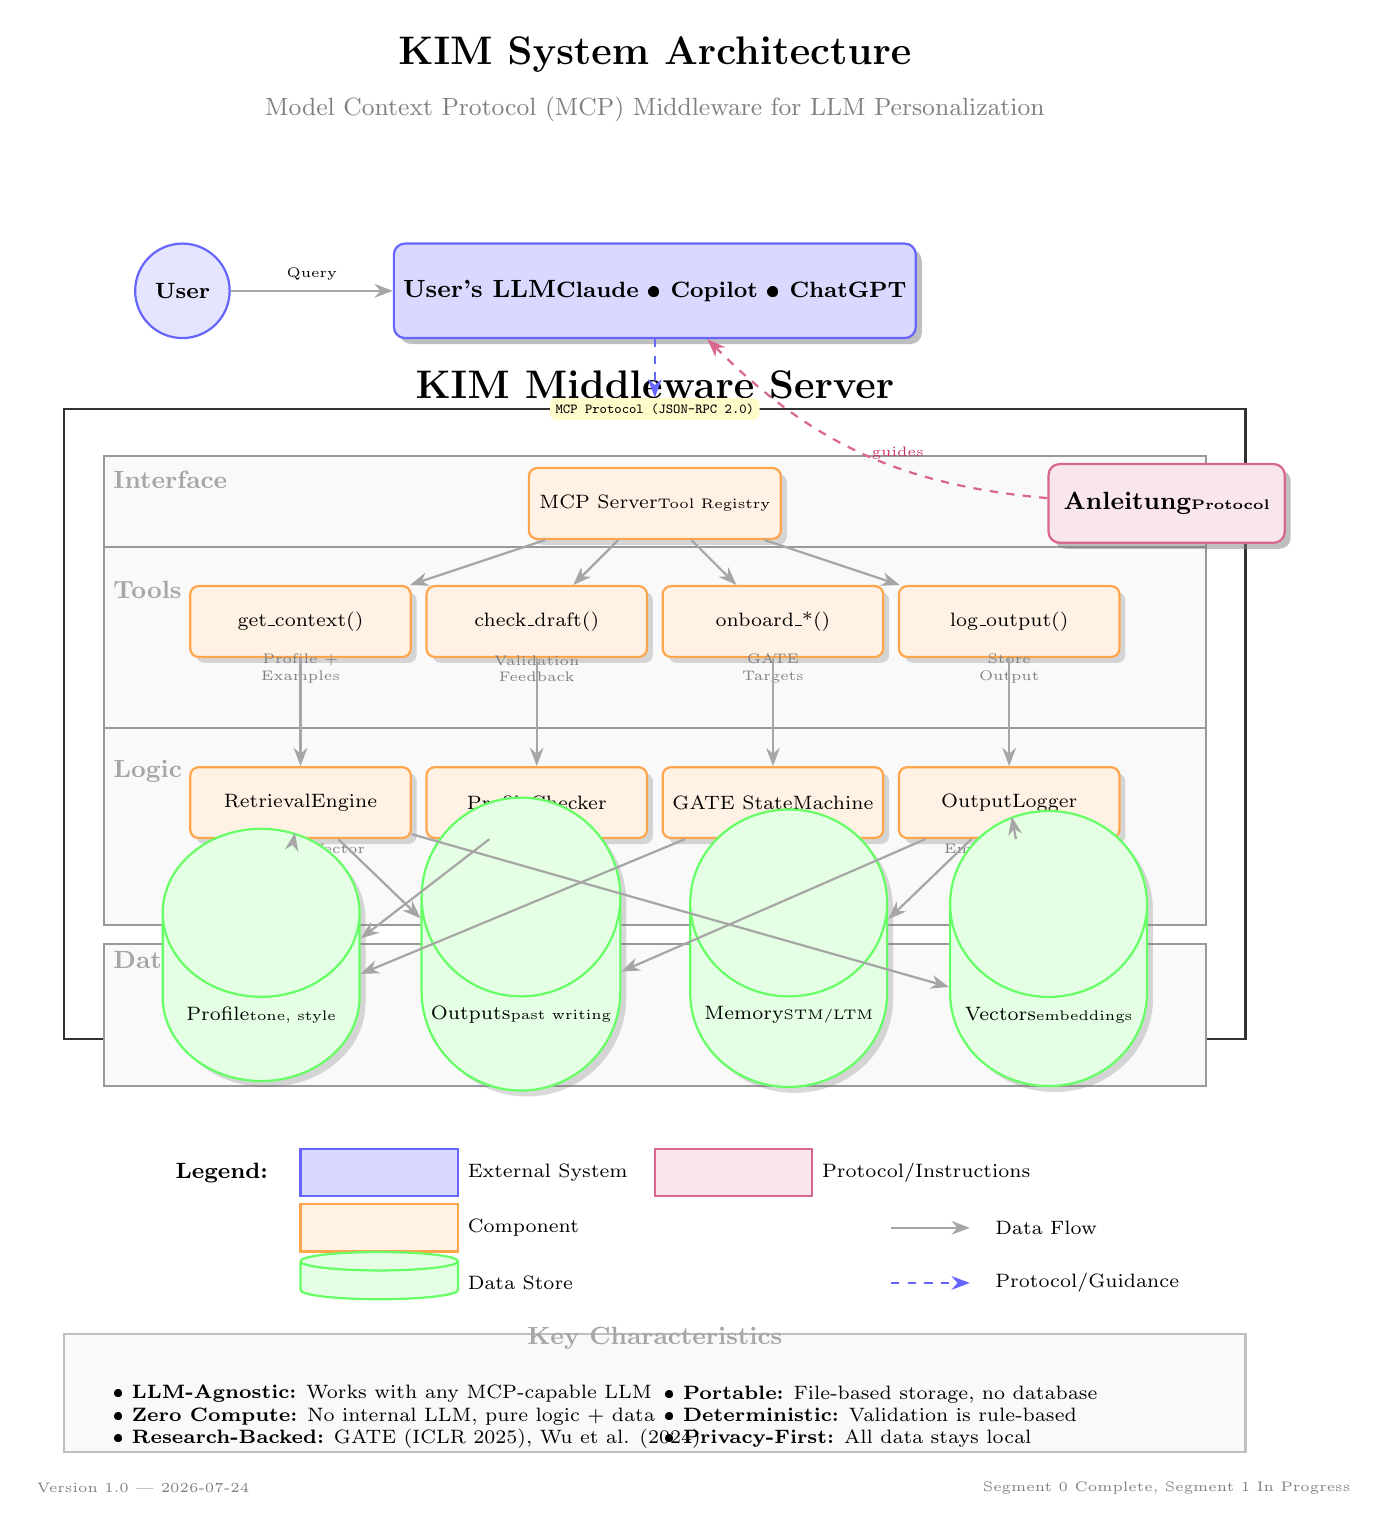
\begin{tikzpicture}[
    node distance=1.5cm,
    % Styles
    actor/.style={
        circle,
        draw=blue!60,
        fill=blue!10,
        thick,
        minimum size=1.2cm,
        font=\footnotesize\bfseries
    },
    external/.style={
        rectangle,
        rounded corners,
        draw=blue!60,
        fill=blue!15,
        thick,
        minimum width=4cm,
        minimum height=1.2cm,
        font=\small\bfseries,
        drop shadow
    },
    layer/.style={
        rectangle,
        draw=gray!80,
        fill=gray!5,
        thick,
        minimum width=14cm,
        minimum height=2.5cm,
        font=\footnotesize
    },
    component/.style={
        rectangle,
        rounded corners=3pt,
        draw=orange!70,
        fill=orange!10,
        thick,
        minimum width=2.8cm,
        minimum height=0.9cm,
        font=\scriptsize,
        drop shadow={opacity=0.3}
    },
    data/.style={
        cylinder,
        draw=green!60,
        fill=green!10,
        thick,
        minimum width=2.5cm,
        minimum height=1cm,
        shape border rotate=90,
        font=\scriptsize,
        drop shadow={opacity=0.3}
    },
    arrow/.style={
        -Stealth,
        thick,
        draw=gray!70
    },
    protocol/.style={
        font=\tiny\ttfamily,
        fill=yellow!20,
        rounded corners=2pt,
        inner sep=2pt
    },
    title/.style={
        font=\Large\bfseries,
        align=center
    },
    legend/.style={
        rectangle,
        draw=black,
        thick,
        minimum width=2cm,
        minimum height=0.6cm,
        font=\scriptsize
    }
]

% Title
\node[title] at (0, 11) {KIM System Architecture};
\node[font=\small, text=gray] at (0, 10.3) {Model Context Protocol (MCP) Middleware for LLM Personalization};

% ═══════════════════════════════════════════════════════════
% EXTERNAL LAYER
% ═══════════════════════════════════════════════════════════

% User
\node[actor] (user) at (-6, 8) {User};

% LLM Client
\node[external] (llm) at (0, 8) {User's LLM\\{\footnotesize Claude • Copilot • ChatGPT}};

% Connection
\draw[arrow] (user) -- node[above, font=\tiny] {Query} (llm);

% ═══════════════════════════════════════════════════════════
% KIM MIDDLEWARE BOX
% ═══════════════════════════════════════════════════════════

% Main container
\node[
    rectangle,
    draw=black!80,
    fill=white,
    thick,
    minimum width=15cm,
    minimum height=8cm,
    label={[font=\Large\bfseries]north:KIM Middleware Server}
] (kimbox) at (0, 2.5) {};

% MCP Protocol indicator
\node[protocol] (mcp) at (0, 6.5) {MCP Protocol (JSON-RPC 2.0)};
\draw[arrow, dashed, blue!60] (llm) -- (mcp);

% ═══════════════════════════════════════════════════════════
% LAYER 1: MCP INTERFACE
% ═══════════════════════════════════════════════════════════

\node[layer, minimum height=1.2cm] (interface) at (0, 5.3) {};
\node[font=\small\bfseries, anchor=west, text=gray!70] at (-7, 5.6) {Interface};

\node[component, minimum width=3.2cm] (mcp_server) at (0, 5.3) {MCP Server\\{\tiny Tool Registry}};

% ═══════════════════════════════════════════════════════════
% LAYER 2: TOOLS (Exposed via MCP)
% ═══════════════════════════════════════════════════════════

\node[layer] (tools) at (0, 3.5) {};
\node[font=\small\bfseries, anchor=west, text=gray!70] at (-7, 4.2) {Tools};

\node[component] (t_context) at (-4.5, 3.8) {get\_context()};
\node[component] (t_check) at (-1.5, 3.8) {check\_draft()};
\node[component] (t_onboard) at (1.5, 3.8) {onboard\_*()};
\node[component] (t_log) at (4.5, 3.8) {log\_output()};

\node[font=\tiny, text=gray, align=center] at (-4.5, 3.2) {Profile +\\Examples};
\node[font=\tiny, text=gray, align=center] at (-1.5, 3.2) {Validation\\Feedback};
\node[font=\tiny, text=gray, align=center] at (1.5, 3.2) {GATE\\Targets};
\node[font=\tiny, text=gray, align=center] at (4.5, 3.2) {Store\\Output};

% ═══════════════════════════════════════════════════════════
% LAYER 3: BUSINESS LOGIC
% ═══════════════════════════════════════════════════════════

\node[layer] (logic) at (0, 1.2) {};
\node[font=\small\bfseries, anchor=west, text=gray!70] at (-7, 1.9) {Logic};

\node[component] (l_retrieval) at (-4.5, 1.5) {Retrieval\\Engine};
\node[component] (l_checker) at (-1.5, 1.5) {Profile\\Checker};
\node[component] (l_gate) at (1.5, 1.5) {GATE State\\Machine};
\node[component] (l_logger) at (4.5, 1.5) {Output\\Logger};

\node[font=\tiny, text=gray, align=center] at (-4.5, 0.9) {BM25 + Vector};
\node[font=\tiny, text=gray, align=center] at (-1.5, 0.9) {Rules};
\node[font=\tiny, text=gray, align=center] at (1.5, 0.9) {Barriers};
\node[font=\tiny, text=gray, align=center] at (4.5, 0.9) {Embed + Index};

% ═══════════════════════════════════════════════════════════
% LAYER 4: DATA STORAGE
% ═══════════════════════════════════════════════════════════

\node[layer, minimum height=1.8cm] (storage) at (0, -1.2) {};
\node[font=\small\bfseries, anchor=west, text=gray!70] at (-7, -0.5) {Data};

\node[data] (d_profile) at (-5, -1.2) {Profile\\{\tiny tone, style}};
\node[data] (d_outputs) at (-1.7, -1.2) {Outputs\\{\tiny past writing}};
\node[data] (d_memory) at (1.7, -1.2) {Memory\\{\tiny STM/LTM}};
\node[data] (d_vectors) at (5, -1.2) {Vectors\\{\tiny embeddings}};

% ═══════════════════════════════════════════════════════════
% CONNECTIONS: MCP Server to Tools
% ═══════════════════════════════════════════════════════════

\draw[arrow] (mcp_server) -- (t_context);
\draw[arrow] (mcp_server) -- (t_check);
\draw[arrow] (mcp_server) -- (t_onboard);
\draw[arrow] (mcp_server) -- (t_log);

% ═══════════════════════════════════════════════════════════
% CONNECTIONS: Tools to Logic
% ═══════════════════════════════════════════════════════════

\draw[arrow] (t_context) -- (l_retrieval);
\draw[arrow] (t_check) -- (l_checker);
\draw[arrow] (t_onboard) -- (l_gate);
\draw[arrow] (t_log) -- (l_logger);

% ═══════════════════════════════════════════════════════════
% CONNECTIONS: Logic to Data
% ═══════════════════════════════════════════════════════════

\draw[arrow] (l_retrieval) -- (d_profile);
\draw[arrow] (l_retrieval) -- (d_outputs);
\draw[arrow] (l_retrieval) -- (d_vectors);

\draw[arrow] (l_checker) -- (d_profile);

\draw[arrow] (l_gate) -- (d_profile);

\draw[arrow] (l_logger) -- (d_outputs);
\draw[arrow] (l_logger) -- (d_memory);
\draw[arrow] (l_logger) -- (d_vectors);

% ═══════════════════════════════════════════════════════════
% ANLEITUNG (Protocol Instructions)
% ═══════════════════════════════════════════════════════════

\node[
    rectangle,
    rounded corners,
    draw=purple!60,
    fill=purple!10,
    thick,
    minimum width=3cm,
    minimum height=1cm,
    font=\small\bfseries,
    drop shadow
] (anleitung) at (6.5, 5.3) {Anleitung\\{\tiny Protocol}};

\draw[arrow, dashed, purple!60] (anleitung) to[bend left=20] node[right, font=\tiny, text=purple!80] {guides} (llm);

% ═══════════════════════════════════════════════════════════
% LEGEND
% ═══════════════════════════════════════════════════════════

\node[font=\footnotesize\bfseries] at (-5.5, -3.2) {Legend:};

\node[legend, fill=blue!15, draw=blue!60] at (-3.5, -3.2) {};
\node[font=\scriptsize, anchor=west] at (-2.5, -3.2) {External System};

\node[legend, fill=orange!10, draw=orange!70] at (-3.5, -3.9) {};
\node[font=\scriptsize, anchor=west] at (-2.5, -3.9) {Component};

\node[legend, fill=green!10, draw=green!60, cylinder, shape border rotate=90, minimum height=0.6cm] at (-3.5, -4.6) {};
\node[font=\scriptsize, anchor=west] at (-2.5, -4.6) {Data Store};

\node[legend, fill=purple!10, draw=purple!60] at (1, -3.2) {};
\node[font=\scriptsize, anchor=west] at (2, -3.2) {Protocol/Instructions};

\draw[arrow] (3, -3.9) -- (4, -3.9);
\node[font=\scriptsize, anchor=west] at (4.2, -3.9) {Data Flow};

\draw[arrow, dashed, blue!60] (3, -4.6) -- (4, -4.6);
\node[font=\scriptsize, anchor=west] at (4.2, -4.6) {Protocol/Guidance};

% ═══════════════════════════════════════════════════════════
% KEY CHARACTERISTICS (Bottom)
% ═══════════════════════════════════════════════════════════

\node[
    rectangle,
    draw=gray!50,
    fill=gray!5,
    thick,
    minimum width=15cm,
    minimum height=1.5cm,
    font=\scriptsize
] (characteristics) at (0, -6) {};

\node[font=\small\bfseries, text=gray!70] at (0, -5.3) {Key Characteristics};

\node[font=\scriptsize, align=left, anchor=west] at (-7, -6.3) {
    \textbullet\ \textbf{LLM-Agnostic:} Works with any MCP-capable LLM\\
    \textbullet\ \textbf{Zero Compute:} No internal LLM, pure logic + data\\
    \textbullet\ \textbf{Research-Backed:} GATE (ICLR 2025), Wu et al. (2024)
};

\node[font=\scriptsize, align=left, anchor=west] at (0, -6.3) {
    \textbullet\ \textbf{Portable:} File-based storage, no database\\
    \textbullet\ \textbf{Deterministic:} Validation is rule-based\\
    \textbullet\ \textbf{Privacy-First:} All data stays local
};

% ═══════════════════════════════════════════════════════════
% VERSION INFO
% ═══════════════════════════════════════════════════════════

\node[font=\tiny, text=gray] at (-6.5, -7.2) {Version 1.0 | 2026-07-24};
\node[font=\tiny, text=gray] at (6.5, -7.2) {Segment 0 Complete, Segment 1 In Progress};

\end{tikzpicture}

\end{document}
